\subsection{bpmprocess/process\_\-monopole.c File Reference}
\label{process__monopole_8c}\index{bpmprocess/process\_\-monopole.c@{bpmprocess/process\_\-monopole.c}}


\subsubsection{Detailed Description}


Definition in file {\bf process\_\-monopole.c}.

{\tt \#include $<$stdio.h$>$}\par
{\tt \#include $<$bpm/bpm\_\-units.h$>$}\par
{\tt \#include $<$bpm/bpm\_\-messages.h$>$}\par
{\tt \#include $<$bpm/bpm\_\-process.h$>$}\par


Include dependency graph for process\_\-monopole.c:\nopagebreak
\begin{figure}[H]
\begin{center}
\leavevmode
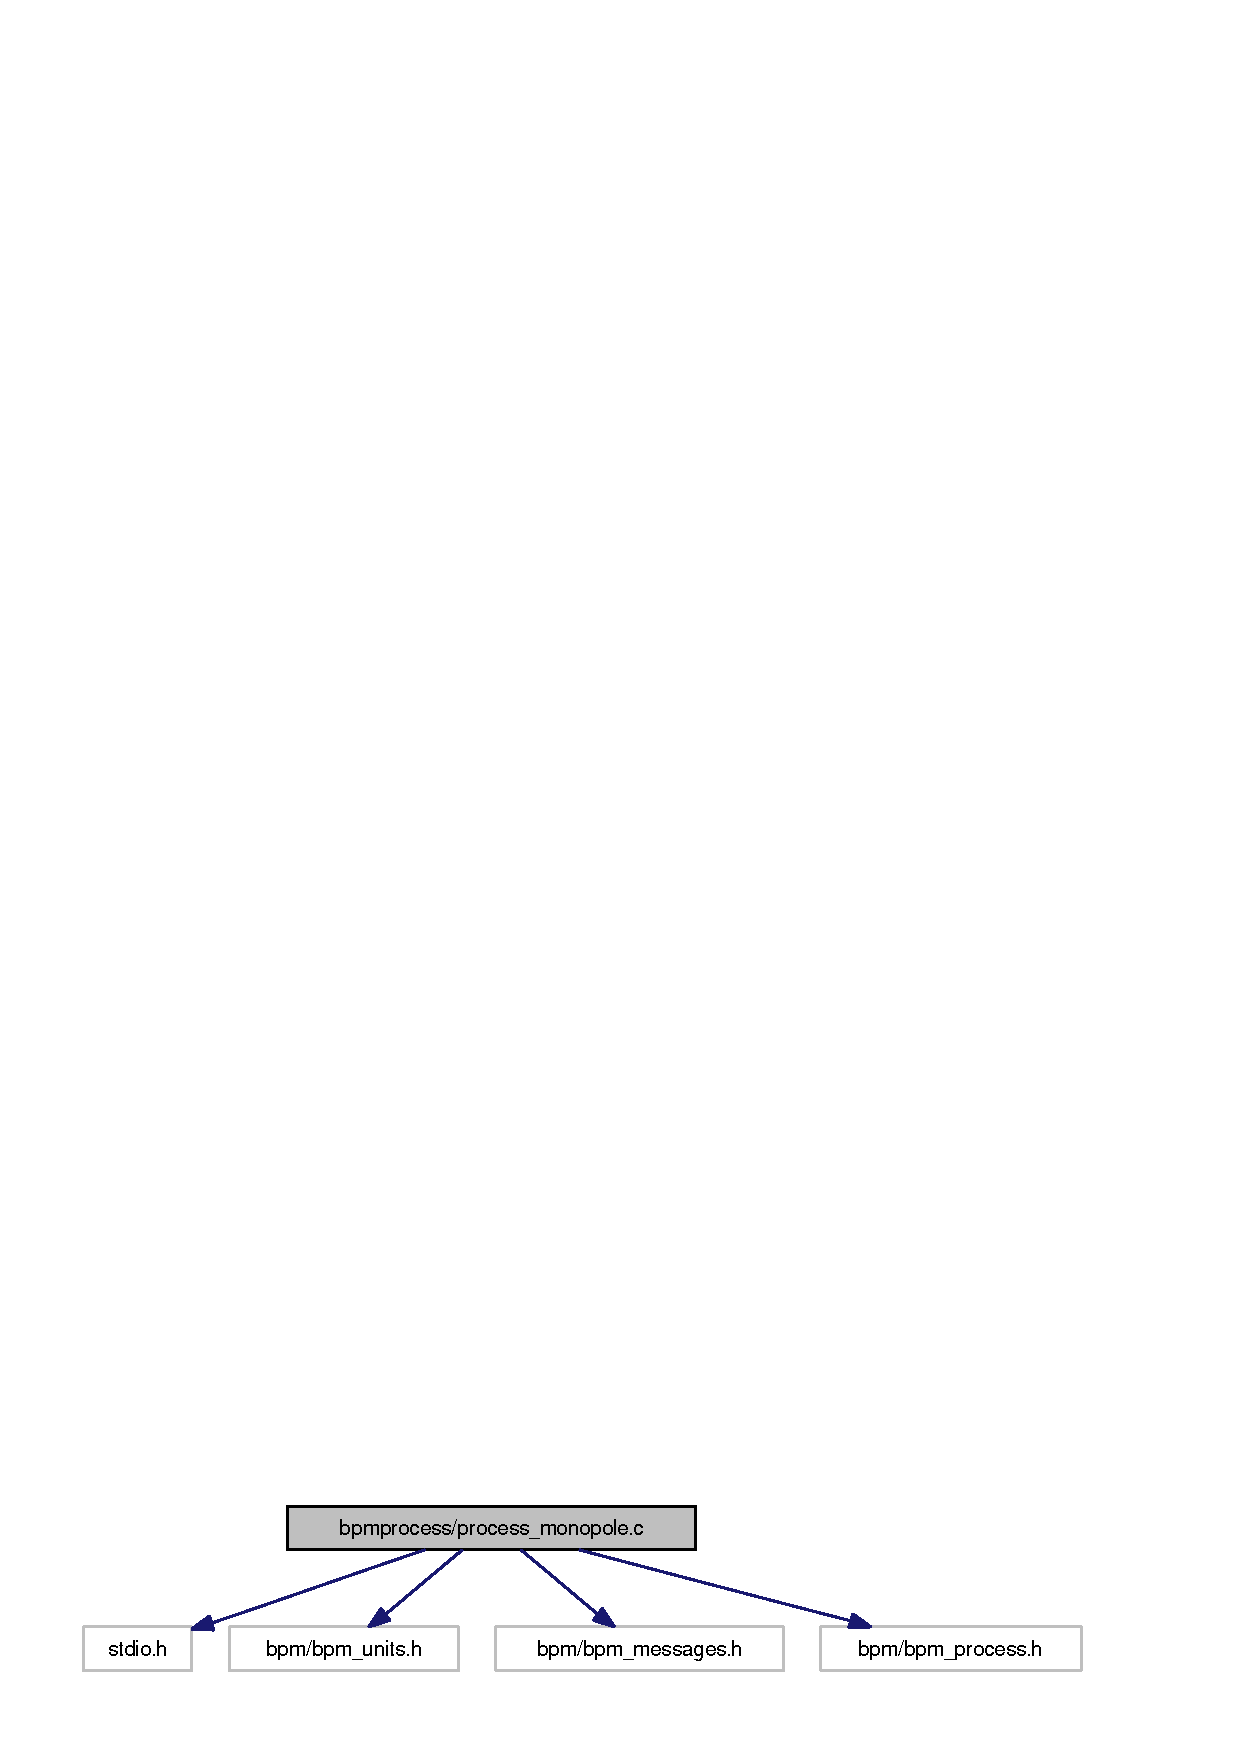
\includegraphics[width=261pt]{process__monopole_8c__incl}
\end{center}
\end{figure}
\subsubsection*{Functions}
\begin{CompactItemize}
\item 
int {\bf process\_\-monopole} ({\bf doublewf\_\-t} $\ast$sig, {\bf bpmconf\_\-t} $\ast$bpm, {\bf bpmcalib\_\-t} $\ast$cal, {\bf bpmproc\_\-t} $\ast$proc, {\bf bpmproc\_\-t} $\ast$trig, unsigned int mode)
\end{CompactItemize}
